%==============================================================================
% Sjabloon poster bachelorproef
%==============================================================================
% Gebaseerd op document class `a0poster' door Gerlinde Kettl en Matthias Weiser
% Aangepast voor gebruik aan HOGENT door Jens Buysse en Bert Van Vreckem

\documentclass[a0,portrait]{hogent-poster}

% Info over de opleiding
\course{Bachelorproef}
\studyprogramme{Toegepaste informatica}
\academicyear{2023-2024}
\institution{Hogeschool Gent, Valentin Vaerwyckweg 1, 9000 Gent}

% Info over de bachelorproef
\title{Efficiënte Integratie van Kalender-API's in Software: Een Gebruikersgerichte Benadering}
\author{Warre Vandenhoucke}
\email{warre.vandenhoucke@student.hogent.be}
\supervisor{Lieven Smits}
\cosupervisor{Jona Decubber (TurnUp)}
\projectrepo{https://github.com/Warrevdh/bachelorproef}

\begin{document}
    
    \maketitle
    
    \begin{abstract}
        Deze poster vat de kernpunten samen van het onderzoek naar de integratie van verschillende kalender-API's in een gebruikersgerichte applicatie, gericht op het verbeteren van de gebruikerservaring en efficiëntie binnen softwareoplossingen.
    \end{abstract}
    
    \begin{multicols}{2} % Dit bepaalt hoeveel kolommen je poster zal hebben; een portret poster is meestal verdeeld in 2 kolommen
        
        \section{Introductie}
        Deze studie onderzoekt de integratie van kalender-API's zoals die van Google Calendar, Microsoft Outlook en Calendly, en richt zich op de optimalisatie van gebruikerservaring en beheer in professionele en persoonlijke omgevingen.
        
        \section{Onderzoeksvragen}
        Het onderzoek richt zich op twee primaire vragen. Ten eerste, hoe kunnen verschillende kalender-API's, zoals die van Google Calendar, Microsoft Outlook en Calendly, effectief worden geïntegreerd in een uniforme gebruikersinterface die zowel functioneel als esthetisch aantrekkelijk is? Ten tweede, welke technische uitdagingen ontstaan bij de integratie van deze meerdere kalenderdiensten en hoe kunnen deze uitdagingen succesvol worden aangepakt om een naadloze gebruikerservaring te garanderen?
        
        \section{Methodologie}
        Dit diagram toont de stapsgewijze aanpak van het onderzoek. Het begint met een Literatuurstudie, waarin belangrijke informatie wordt verzameld en geanalyseerd om een grondig begrip te krijgen van wat er al bekend is over kalender-API's. Daarna wordt een Proof of Concept (PoC) ontwikkeld. Dit is een eerste versie van de oplossing die wordt opgezet en getest om de werking ervan te evalueren. Vervolgens worden de resultaten onderzocht in de fase Analyse van de Resultaten, waarbij de functionaliteit van de PoC en de feedback van gebruikers worden beoordeeld. De laatste stap is de Conclusie, waarin de belangrijkste bevindingen worden samengevat en overwogen wordt wat in toekomstig onderzoek nog kan worden verkend. Elk deel van dit proces is cruciaal om betrouwbare resultaten en aanbevelingen te kunnen doen.
        
        \begin{center}
            \captionsetup{type=figure}
            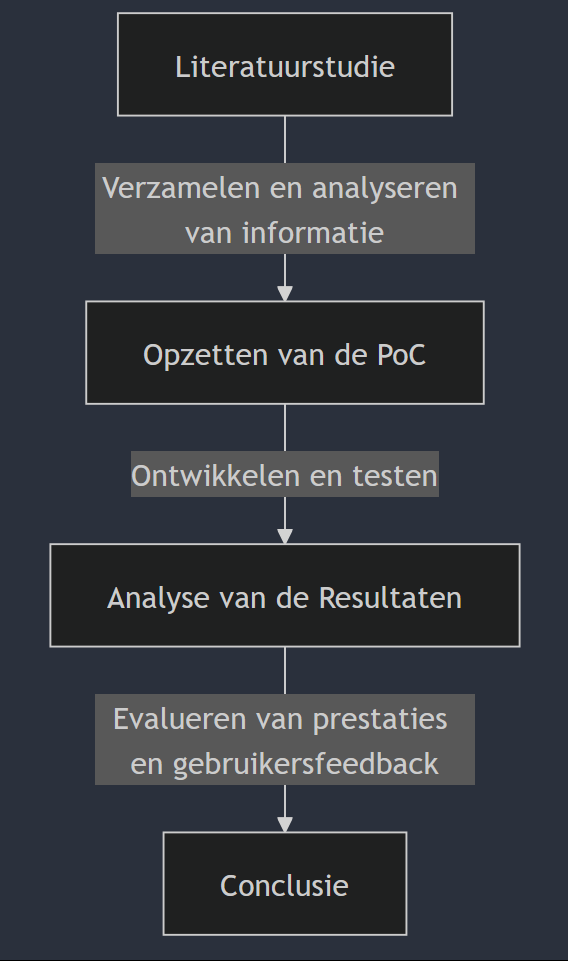
\includegraphics[width=0.3\linewidth]{flowchart}
            \captionof{figure}{Flowchart van de onderzoeksmethodologie}
        \end{center}
        
        \section{Conclusies}
        De integratie van kalender-API's biedt significante verbeteringen in de efficiëntie van tijdbeheer en verhoogt de consistentie en toegankelijkheid van kalendergegevens over verschillende platforms heen.
        
        \section{Toekomstig onderzoek}
        Toekomstig onderzoek kan zich richten op de integratie van geavanceerde machine learning technieken om gebruikersgedrag te voorspellen en de kalenderinterface verder te personaliseren. Daarnaast zijn uitbreidingen naar mobiele platforms en onderzoek naar real-time synchronisatie methoden waardevolle volgende stappen.
        
    \end{multicols}
\end{document}
